% Options for packages loaded elsewhere
\PassOptionsToPackage{unicode}{hyperref}
\PassOptionsToPackage{hyphens}{url}
%
\documentclass[
]{article}
\usepackage{amsmath,amssymb}
\usepackage{lmodern}
\usepackage{ifxetex,ifluatex}
\ifnum 0\ifxetex 1\fi\ifluatex 1\fi=0 % if pdftex
  \usepackage[T1]{fontenc}
  \usepackage[utf8]{inputenc}
  \usepackage{textcomp} % provide euro and other symbols
\else % if luatex or xetex
  \usepackage{unicode-math}
  \defaultfontfeatures{Scale=MatchLowercase}
  \defaultfontfeatures[\rmfamily]{Ligatures=TeX,Scale=1}
\fi
% Use upquote if available, for straight quotes in verbatim environments
\IfFileExists{upquote.sty}{\usepackage{upquote}}{}
\IfFileExists{microtype.sty}{% use microtype if available
  \usepackage[]{microtype}
  \UseMicrotypeSet[protrusion]{basicmath} % disable protrusion for tt fonts
}{}
\makeatletter
\@ifundefined{KOMAClassName}{% if non-KOMA class
  \IfFileExists{parskip.sty}{%
    \usepackage{parskip}
  }{% else
    \setlength{\parindent}{0pt}
    \setlength{\parskip}{6pt plus 2pt minus 1pt}}
}{% if KOMA class
  \KOMAoptions{parskip=half}}
\makeatother
\usepackage{xcolor}
\IfFileExists{xurl.sty}{\usepackage{xurl}}{} % add URL line breaks if available
\IfFileExists{bookmark.sty}{\usepackage{bookmark}}{\usepackage{hyperref}}
\hypersetup{
  pdftitle={One if by land, and two if by sea: Cross-domain contests and the escalation of international crises},
  hidelinks,
  pdfcreator={LaTeX via pandoc}}
\urlstyle{same} % disable monospaced font for URLs
\usepackage[margin=1in]{geometry}
\usepackage{longtable,booktabs,array}
\usepackage{calc} % for calculating minipage widths
% Correct order of tables after \paragraph or \subparagraph
\usepackage{etoolbox}
\makeatletter
\patchcmd\longtable{\par}{\if@noskipsec\mbox{}\fi\par}{}{}
\makeatother
% Allow footnotes in longtable head/foot
\IfFileExists{footnotehyper.sty}{\usepackage{footnotehyper}}{\usepackage{footnote}}
\makesavenoteenv{longtable}
\usepackage{graphicx}
\makeatletter
\def\maxwidth{\ifdim\Gin@nat@width>\linewidth\linewidth\else\Gin@nat@width\fi}
\def\maxheight{\ifdim\Gin@nat@height>\textheight\textheight\else\Gin@nat@height\fi}
\makeatother
% Scale images if necessary, so that they will not overflow the page
% margins by default, and it is still possible to overwrite the defaults
% using explicit options in \includegraphics[width, height, ...]{}
\setkeys{Gin}{width=\maxwidth,height=\maxheight,keepaspectratio}
% Set default figure placement to htbp
\makeatletter
\def\fps@figure{htbp}
\makeatother
\setlength{\emergencystretch}{3em} % prevent overfull lines
\providecommand{\tightlist}{%
  \setlength{\itemsep}{0pt}\setlength{\parskip}{0pt}}
\setcounter{secnumdepth}{5}
\usepackage{tikz}
\usepackage{pgfplots}
\pgfplotsset{compat=newest}
\usetikzlibrary{plotmarks}
\usetikzlibrary{arrows.meta}
\usepgfplotslibrary{patchplots}
\usepackage{grffile}
\usepackage{caption}
\usepackage[utf8]{inputenc}
\usepackage[doublespacing]{setspace}
\usepackage{setspace}
\AtBeginEnvironment{tabular}{\singlespacing}
\usepackage{float}
\usepackage{multirow}
\usepackage{booktabs}
\usepackage{longtable}
\usepackage{array}
\usepackage{multirow}
\usepackage{wrapfig}
\usepackage{float}
\usepackage{colortbl}
\usepackage{pdflscape}
\usepackage{tabu}
\usepackage{threeparttable}
\usepackage{threeparttablex}
\usepackage[normalem]{ulem}
\usepackage{makecell}
\usepackage{xcolor}
\ifluatex
  \usepackage{selnolig}  % disable illegal ligatures
\fi
\newlength{\cslhangindent}
\setlength{\cslhangindent}{1.5em}
\newlength{\csllabelwidth}
\setlength{\csllabelwidth}{3em}
\newenvironment{CSLReferences}[2] % #1 hanging-ident, #2 entry spacing
 {% don't indent paragraphs
  \setlength{\parindent}{0pt}
  % turn on hanging indent if param 1 is 1
  \ifodd #1 \everypar{\setlength{\hangindent}{\cslhangindent}}\ignorespaces\fi
  % set entry spacing
  \ifnum #2 > 0
  \setlength{\parskip}{#2\baselineskip}
  \fi
 }%
 {}
\usepackage{calc}
\newcommand{\CSLBlock}[1]{#1\hfill\break}
\newcommand{\CSLLeftMargin}[1]{\parbox[t]{\csllabelwidth}{#1}}
\newcommand{\CSLRightInline}[1]{\parbox[t]{\linewidth - \csllabelwidth}{#1}\break}
\newcommand{\CSLIndent}[1]{\hspace{\cslhangindent}#1}

\title{\singlespacing One if by land, and two if by sea: Cross-domain contests and the escalation of international crises}
\author{J Andr\(\'{e}\)s Gannon\footnote{Email: \texttt{jagannon@hks.harvard.edu}. Web: \texttt{jandresgannon.com}. \newline The author wishes to thank Erik Gartzke and Jon Lindsay who were Principal Investigators on Office of Naval Research Grant N00014-14-1-0071 and the Department of Defense Minerva Research Initiative grant that organized the data collection for this project. Rex Douglass and Thomas Leo Scherer are responsible for the underlying ontology and event data and ICB project managers Jonathan Wilkenfeld and David Quinn oversaw the coding effort. Tom Brailey, David McCrum, James McCullough, Cole Reynolds, Cailen Rodriguez, Woong Suh, and Erin Werner provided excellent research assistance. The author is also grateful for constructive feedback from Shannon Carcelli, Jasen Castillo, James Fowler, Patrick Hulme, Nadiya Kostyuk, Igor Kovak, Kendrick Kuo, Nicole Letourneau, Sara Plana, Laura Resnick Samotin, Rachel Schoner, Ryan Shandler, and Sanne Verschuren. Any opinions, findings, or recommendations do not necessarily reflect the view of the Office of Naval Research. Data and code can be found at \texttt{https://github.com/CenterForPeaceAndSecurityStudies/ICBdomains}.}\\
Belfer Center for Science and International Affairs\\
Harvard Kennedy School}
\date{May 04, 2022}

\begin{document}
\maketitle
\begin{abstract}
\singlespacing \noindent New domains of military conflict like space and cyber arguably increase opportunities for conflict across, as well as within, domains. Cross-domain conflict is thus seen by many as an emerging source of international instability. Yet, existing systematic empirical research has little to say about how domains interact. This study introduces a new dataset of the domains in which nations took military action during 412 international crises between 1918 and 2015. Analysis of these data yields several surprises. Far from being rare, cross-domain interactions are the modal form of conflict in crises during this period. Nor is cross-domain conflict ``new:'' crises that play out in more than one domain were about as frequent (proportionately) in decades past as they are today. Cross-domain crises are also less violent and of no greater duration than crises between belligerents using similar means. This study thus presents evidence that fears about cross-domain escalation are empirically unsubstantiated.
\end{abstract}

\newpage

\hypertarget{introduction}{%
\section{Introduction}\label{introduction}}

Increased technological sophistication has given rise to new modes of conflict as states acquire a growing number of options through which to confront one another. During the advent of each new conflict domain, practitioners scramble to update military strategy and technology to keep up with the now irreparably transformed landscape of war. General Perkins, Senior Commander of Training and Doctrine Command, noted that the Cold War featured ``ground forces fighting ground forces, air forces fighting air forces. Cyber didn't even exist when I was a lieutenant. What's happening now is those lines are blurring between those domains\ldots So what we're seeing is the ability to take an activity in one domain and produce an effect or dominate another domain.''\footnote{quoted in Tan (2017).} There is little consensus about whether to sound the alarm about dangerously escalatory cross-domain interactions (Pettyjohn and Wasser 2019) or to caution against excess concern (Borghard and Schneider 2019). There also remains considerable ambiguity about whether recent cases of cross-domain conflict are emblematic of the future of warfare (Horowitz 2020), or are at most variations on a more durable set of themes (Gannon et al. 2021). As so often occurs, the question is ``how new is new?'' Using a new dataset on the domains in which states took military action during international crises over the past century, this paper finds cross-domain military contests are neither new nor cause for alarm.

While recent events have motivated a growing interest in understanding the settings in which states take military action and the consequences those choices have for international stability, the larger context of cross- or multi-domain conflict has not been studied systematically. In part, this is due to limited empirical data concerning the conduct of conflict. While scholars have developed numerous detailed datasets of participants, duration, and outcomes to understand conflict, empirically-oriented research concerning where contests take place, within which domain, has only recently received attention (Lindsay and Gartzke 2019; Douglass et al. 2022). Researchers typically frame their inquiries around particular emerging technologies (Sechser, Narang, and Talmadge 2019) or operations within individual domains, unable to address more formative questions about how domains interact (Allen and Martinez Machain 2017, 2018; Lupton 2020).\footnote{For work that does look at cross-domain interaction, see Martinez Machain (2015), Macdonald and Schneider (2019), and Post (2019).}

This paper takes an inductive, data-driven approach to identify spatial and temporal patterns in the military domains in which states operate during conflict as well as the relationship between cross-domain interactions and the intensity and duration of international crises. This study adopts a commonly agreed upon understanding shared by practitioners and scholars that contains the traditional domains of land, air, and sea as well as the recent domains of space, cyber, and weapons of mass destruction (WMD).\footnote{While WMD is rarely a distinct military branch and has geographic overlap with the other domains, they do represent a distinct domain in how actors think about them in the international context. My concern here is less to get domains ``right'' and more to expose the diversity of options for conflict setting.} In doing so, the study develops and introduces a novel dataset of the military domains in which 1,282 crisis actors operated during 425 international crises from 1918 to 2015. These data expand on the familiar and well-regarded International Crisis Behavior dataset (Brecher and Wilkenfeld 2000).

This paper introduces new data that adjudicates between the deterrence and spiral models of conflict, with four main findings. First, cross-domain conflict is prevalent. Some degree of cross-domain military action occurs in 58\% of crises over the past century, with 23\% of crises involving completely dissimilar military actions by belligerents. Second, cross-domain conflict is not novel: the rate of ``cross-domainness'' has remained more-or-less constant over the past century despite the accumulation of new military domains during this time period. The number of domains available does not itself seem to have triggered a greater reliance on cross-domain operations. Third, crises in which belligerents engage in cross-domain military conflict are no more escalatory than crises where conflict remains within a given domain. Indeed, cross-domain conflicts in crises actually appear slightly less violent than conflicts within domains. Finally, cross-domain conflict in crises does not endure appreciably longer than crises in which states respond with like-means. Taken together, these findings seem to support optimistic interpretations of the effects of cross-domain conflict and to mitigate against pessimistic fears. While data on the more salient new domains like cyber remains limited at this time and these domains may be distinct when it comes to likely casualties and the types of actors that engage, insights about cross-domain interactions in more traditional military domains should help to inform theories of conflict as they are being developed and applied to more novel domains.

This paper is organized into four sections. Section 2 outlines existing thinking concerning the domains in which states fight and details the theoretical debate between cross-domain pessimists and optimists, as applied to the intensity and duration of international crises. Section 3 provides an empirical test of these contrasting theories by introducing a novel dataset of the military domains in which states operated during international crises since 1918, finding that cross-domain conflicts are less violent and no longer in duration than conflicts where both sides engage in the same military domains. Section 4 concludes with the implications of these findings for questions related to conflict dynamics.

\hypertarget{the-dialectic-across-domains}{%
\section{The Dialectic Across Domains}\label{the-dialectic-across-domains}}

A growing number of studies seek to address the effect on escalation of \textit{how} conflicts are fought (Kreps and Schneider 2019; Cunningham 2020). Despite manifest interest, however, there is little agreement about how to conceptualize and categorize the means by which nations fight. One approach to differentiating the means of conflict is in terms of the domains in which contests take place. The term ``domain'' is used here loosely to refer to land, air, sea, WMD, space, and cyber. Because they can be distinguished from one another by technology, tactics, geography, and purpose, domains here represent a useful starting point for thinking about differences in the ways that nations choose to fight, and how these differences affect observable attributes of conflict, such as duration or intensity (Lindsay and Gartzke 2019).\footnote{Some have questioned the utility of conceptualizing these domains as distinct, especially as new domains like space and cyber increasingly play the role of supplementing rather than supplanting operations in more traditional domains (Libicki 2012).}

If the problem of the security dilemma is to decide whether a particular response to an adversary's behavior will deter or escalate, the problem as applied to the conduct of an actual conflict is whether the military means one chooses determines the likelihood of escalation. Even where recent empirical research has made headway in identifying the ownership and use of new modes of warfare, the efforts are often contained to a single capability or domain. Evaluations of the importance of actions in domains has recently shifted to theorizing about interactions \emph{across} domains (Lindsay and Gartzke 2019). There is suspicion that cross-domain interactions are more prevalent now because there are more (and newer) domains in which states operate. If domains differ from one another in the constraints (and opportunities) they offer concerning power projection, movement, coordination, casualty risk, and cost -- all these factors could produce unique cross-domain dynamics regarding conflict intensity and duration (Lindsay and Gartzke 2020, 9--10). Researchers and policymakers have expressed concerns that new tools of warfare may embolden revisionist forces in world affairs (Hicks and Friend 2019), although skepticism about the novelty and efficacy of these ``new'' forms of warfare has also cast some doubt on those concerns (Gannon et al. 2021). Empirical evidence, however, remains limited due in large part to the very novelty and putative heterogeneity of these emerging domains (Mawdsley 2016).

``A ship's a fool to fight a fort.''\footnote{The quote is generally (mis)credited to Admiral Lord Horatio Nelson, RN (Ferreiro 2016).} But is it wiser for a commander, or a nation, to attack a fort with another fort? Interpreting ``foolish'' actions as those that increase a conflict's violence and/or duration, perhaps unnecessarily, this study identifies two sets of disparate expectations about cross-domain interactions. Despite contrasting predictions from the literature best characterized by the classical dialectical debate between deterrence theory and the spiral model, both perspectives share the assumption that the manner in which states engage in a crisis influences whether it is resolved peacefully (Kydd 1997). For the spiral model, the threat of punishment backfires and causes one's opponent to escalate while for the deterrence model, the threat of punishment elicits compliance (Jervis 1976; Priebe 2015). These perspectives thus differ in whether demonstrations of resolve and/or capability succeed or fail when they involve transporting actions to a military domain in which one's opponent is not operating. This section elucidates these opposing theories and develops contrasting hypotheses that the new empirical evidence on cross-domain military contests will then test.

\hypertarget{cross-domain-escalation}{%
\subsection{Cross-domain escalation}\label{cross-domain-escalation}}

Crises in which actors interact in dissimilar military domains may be more violent and/or last longer because cross-domain interactions complicate interpretations of proportionality and the scope of disputed stakes, thus contributing to misperceptions of capability or resolve (Morrow 2019). If a belligerent taking action with 100 ground troops is met with a defender deploying 1000 ground troops, the belligerent could reasonably interpret the defender's action as a ``raise'' indicating the defender places a high value on the issue(s) in dispute. But if the defender responds to a deployment of 100 troops with 10 aircraft, it is less clear whether that is a raise, or instead is an effort to achieve something different, such as saving face. Schelling describes the risk of a hypothetical example where the US responds to Soviet missiles in Cuba by quarantining Vladivostok. Because there is ``a tendency to keep things in the same currency, to respond in the same language,'' cross-domain conflict makes it difficult for actors to ascertain their opponents resolve (Schelling 1966, 147). Cross-domain conflict presents actors with an ``apples-to-oranges'' comparison, making it more difficult potentially to assess relative resolve or an opponent's value for the issue(s) at stake. This injection of (additional) ambiguity could make a negotiated settlement more difficult by clouding evaluations of the bargaining range.

Uncertainty can cause, or worsen, a contest by creating incompatible expectations about a contest's likely outcome or utility (Gartzke 1999). Asymmetry in the military domains in which belligerents are taking actions can be a source of that uncertainty. Cross-domain interactions may be perceived by the adversary as shifting to a domain where one actor has escalation dominance because of a relatively \textit{low} value for the stakes of the conflict. Since each military domain has different strengths and weaknesses concerning outcomes like credibility, costs, signaling, and relative war fighting ability, operating in a different domain that one's adversary may signal a difference in tolerance for cost or risk (Gartzke et al. 2017). One can represent this aspect of military domains in terms of a game of rock, paper, scissors, where each domain's characteristics bring advantages against some of an opponent's possible domains, but disadvantages against others (Lindsay and Gartzke 2019, 16). In discussing the dangers of Chinese power projection from land, former US National Security Adviser H.R. McMaster (2016) advised practitioners to recognize the synergy ``between joint force capabilities and how, you know, really joint operations - it's rock, paper, scissors, you know? So if you can - if you have all of those tools available - maritime, aerospace, cyberspace, land capabilities - then you're able to pose that enemy with multiple dilemmas.''

While presenting your enemy with multiple dilemmas --- responding to your adversaries ``rock'' with ``paper'' --- may help you win a contest, it could also produce an incentive for your opponent to do the same --- respond again with ``scissors'' --- thus encouraging escalation (Talmadge 2017). It has been argued that responding in-kind --- playing rock against rock --- should be de-escalatory because it represents a symbolic gesture to opt against one's most efficient response (paper), as doing so would require the opposing side to engage in a new, even more efficient response (scissors). If an actor has a comparative advantage in a domain in which their opponent is not taking action, opting not to reap the benefits of conflict in that domain represents a refusal to escalate.\footnote{An empirical test of this argument requires data on the domains in which an actor \emph{could} take military action. Although that data is not introduced in this paper, it is noted as an important area for further inquiry.} By responding in-kind, states can agree to call it a draw in a way that represents an explicit or tacit compromise (Carson 2016). Conversely, engaging in a new military domain may unintentionally create an ``escalatory updraft'' if the opponent misinterprets what should be a tit-for-tat response that ends aggression with one that instead escalates it (O'Neill 1991, 104). Taking action in a new domain may help one side secure victory by representing a reduction in cost, but the very logic of escalation dominance that generates that outcome also means interacting in the new domain constitutes a (relative) increase in cost for one's opponent, with adverse consequences for the likelihood of a peaceful settlement (Mehta 2019). Cheap and easy can be attractive, but it sends mixed messages. An opponent may be cowed by superior capabilities across domains, but they may also be encouraged by implicit evidence of an opponent's unwillingness to pay the high(er) price of sticking it out, within a given domain.

~~\textbf{\textit{Pessimist Hypothesis 1:}}\textit{ Interstate crises in which belligerents act in dissimilar military domains should be more violent than those in which belligerents act in similar military domains.}

~~\textbf{\textit{Pessimist Hypothesis 2:}}\textit{ Interstate crises in which belligerents act in dissimilar military domains should be longer in duration than those in which belligerents act in similar military domains.}

States may often share the assumption that opponents will ``follow precedent by responding in kind with similar weapons against a similar target set'' (Warden 2018, 24). If so, then failing to respond in kind (within domains) risks un-calibrated escalation. Scholars have raised this concern in the US-China context in arguing that ``war at sea could thus quickly become a war on land, potentially even raising risks of nuclear escalation if the US starts to erode potential capabilities relevant to China's nuclear arsenal'' (Talmadge 2019, 880--81).

\hypertarget{cross-domain-deterrence}{%
\subsection{Cross-domain deterrence}\label{cross-domain-deterrence}}

Just as deterrence and the spiral model make contrasting claims from similar priors, the opposite (optimist) logic could also be at play in assessing cross-domain escalation. Crises involving states taking military actions in dissimilar domains could be less likely to escalate by communicating a change in the stakes and a willingness to escalate or by giving one side the upper hand if conflict actually breaks out (Rovner 2020). The apples-to-oranges analogy may be backwards; rather than creating confusion about resolve or the opponent's evaluation of the stakes, a willingness to play a different game may signal that it is better to try to resolve the conflict rather than fighting. Moving to a new domain may provide a way for an actor to simultaneously signal resolve and restraint in a way that reduces the intensity and duration of a conflict that is logically similar to coordinating focal points, as witnessed with covert operations (Carson and Yarhi-Milo 2017) or firebreaks as evidenced experimentally with cyber attacks (Kreps and Schneider 2019).

Rather than simply thinking of military domains as playing rock, paper, or scissors, the different virtues of various domains also creates distinctions in what it means to ``play'' one of them. Threats differ from forward deployments which further differ from seizing territory or discharging a rocket (Lai 2004). Operating in a new domain could deter rather than inflame by providing an avenue for graduated escalation. Reinforcing an army unit by putting bombers on alert or forward deploying a naval unit could be an incremental way of signaling resolve and a willingness to escalate without necessarily increasing the number of army troops already in context with the enemy (Slantchev 2005). Using the same assumption of escalation dominance, action in a new domain in which your opponent is not operating because they do not have escalation dominance in that domain can be a costly signal that makes a negotiated settlement more likely (Quek 2013). In the same way that children on a playground may yell `hotter' or `colder' as their blindfolded classmate tries to find some object, operating in new domains can add credibility to verbal statements about whether an actor perceived an offered negotiation as preferable to continuing to fight (Mastro 2011). Furthermore, deterrence may work not because of mutual vulnerability, but because of one-sided fear about overwhelming punishment (Lieber and Press 2020). If operating in a new domain during a crisis indicates a state's willingness to take action in a domain where it has escalation dominance then this may convey that the state is willing to incur higher costs, so that an opponent is better off backing down.

~~\textbf{\textit{Optimist Hypothesis 1:}}\textit{ Interstate crises in which belligerents act in dissimilar military domains should be less violent than those in which belligerents act in similar military domains.}

~~\textbf{\textit{Optimist Hypothesis 2:}}\textit{ Interstate crises in which belligerents act in dissimilar military domains should be shorter in duration than those in which belligerents act in similar military domains.}

There are numerous historical examples illustrating this logic. In 1969, President Richard Nixon placed US nuclear bombers on alert in an attempt to signal a willingness to gradually escalate or de-escalate in response to Soviet and North Vietnamese actions (Operation Giant Lance) (Burr 2005). The example conforms with existing signaling theories in finding that some domains are better suited to turning the dial incrementally rather than all at once (Post 2019). Secretary of Defense McNamara had a similar rationale in advocating ``flexible response.'' In the event of limited Soviet aggression, advocates hoped that a more credible threat of utilizing limited nuclear force would be sufficient to persuade the Soviet Union to back down (Duffield 1991).\footnote{Experts disagree about whether Kennedy actually believed in, and would have implemented, ``flexible response'' or whether it was political theater (Gavin 2001). The example is meant to simply illustrate the logic used by proponents of the policy.} Similarly, a ceasefire was declared between Israel and Hamas the day after Israel responded to Hamas' cyberattacks with an airstrike (Morris, Eglash, and Balousha 2019). The very conditions that create a threat of immediate escalation in a cross-domain response make such an action conducive to medium and long-term de-escalation. By showing that an opponent has crossed a red line with the intensity of their aggression, a cross-domain response could convey that there are significant costs to be had if an opponent fails to pull back (Altman 2018).

Cross-domain interactions may not themselves be a direct cause of escalation (or de-escalation), but rather might represent an observable indicator for different motives to escalate in a way that masks the stakes. States with more to lose may be more willing to escalate, but cross-domain interactions may communicate this poorly, since doing so relies on an opponent identifying the costs of an adversary's action when that same action would generate different costs for themselves (Lupton 2018). Rather than try to empirically identify whether the underlying causes of cross-domain interactions directly or indirectly determine conflict intensity, the hope here is to shed light on the association between the use of these domains and crisis outcomes, whatever their origins.

\hypertarget{empirics-and-research-design}{%
\section{Empirics and Research Design}\label{empirics-and-research-design}}

This section lays out the research design, empirical strategy, and data to test they hypotheses detailed above. The primary empirical contribution of the study is the introduction of a new dataset detailing the domains in which military actions or conflict occurred during 425 distinct crises from 1918 to 2015. The new data contain information on 1,282 crisis actors, the majority of which are states.\footnote{International organizations and non-state actors sometimes deploy military or quasi-military capabilities like peacekeepers or foreign aid distributors. The military logic of these actors is not addressed here, but the data is available for future work.} This crisis-domain dataset represents a unique source of information on the domains in which militaries operate during conflict.

The data were developed in three distinct steps. First, a research team event coded the 425 crises in the International Crisis Behavior (ICB) dataset, identifying the military domains in which crisis actors acted. Second, the data were re-organized at the crisis-dyad level using pre-existing work on ICB crisis-dyads as well as new codings for crisis-dyads post-2010 -- the most recent year coded in pre-existing efforts. Third, a new measure was created of the dissimilarity of the domains in which each side in the crisis took military actions, a numeric measure referred to as ``cross-domainness.'' These steps are discussed in greater detail below.

\hypertarget{event-coding}{%
\subsubsection{Event coding}\label{event-coding}}

A research team extended the ICB dataset by gathering extensive data on how actors interacted during crises.(This is a subset of the broader project ICBe dataset. This paper's unique contribution involved re-coding the military domains, the two sides, and the measure of cross-domainness. For the larger event dataset and more detailed explanation of the underlying ontology, see Douglass et al. 2022.) A crisis is defined as an international event where 1) an actor perceives a threat to one or more of its basic values, 2) there is a finite timeline for responding, and 3) there is a heightened probability of military hostilities (Brecher and Wilkenfeld 2000). A crisis can escalate to an actual military dispute, but that does not always happen. This provides variation in the dependent variable, allowing comparison of cases where a crisis did violently escalate to cases where the crisis did not. The dataset introduced contains detailed information on the military domains used by each actor during every international crisis. As such, the unit of analysis is the crisis-actor and the newly coded variables are binary values representing whether that actor took military action in a given domain during the crisis.

Project coders based their coding decisions on the ICB crisis narratives that provide qualitative descriptions of each crisis. Unlike other event datasets that pool from multiple news sources with various data generating processes, the ICB narratives are written in a systematic fashion, contain comparable levels of detail, and were written by the same research team at the University of Maryland. The quality of these narratives reduces the risk that variation among crisis variables is due to variation in the measurement process. For example, more recent crises do not have more detailed crisis narratives (a problem for the reporting of militarized interstate disputes captured by scraping news sources). The ICB narratives are also accompanied by the detailed ICB dataset, allowing the newly coded domain variables to be integrated into the broader ICB project.

The data created here involves the domains in which states took actions during international crises. The domains in which a crisis-actor can take a military action based on the military units that undertook the action, as described in Table \ref{tab:domains}. The coders distinguished actions, speech acts, and thoughts for consistency with pre-existing event datasets like CAMEO and Phoenix (Schrodt et al. 2005; Althaus et al. 2020). Actions are defined as physical acts performed by one of more actors. Examples of military actions include raises in alert level, mobilizations, fortification, military exercises, weapons tests, deployments, shows of force, blockades, border violations, attacks, invasions, and bombardments. Planning to take an action does not constitute an action unless this action is subsequently carried out. For example, a state making a verbal threat to send tanks into a neighboring country is not coded as a ground action unless the state deployed, attacked, or otherwise took a subsequent physical action with land units.

\begin{table}[]
\caption{Military domains coded for each crisis actor. Codings are binary with 1 indicating the actor took an action in that domain during the crisis and 0 otherwise.}
\label{tab:domains}
\centering
\begin{tabular}{|l|l|}
\hline
\textbf{Domain} & \textbf{Description} \\
\hline
Air & Bombers, fighters, and missiles \\
Cyber & Information operations and cyber disruption \\
Land & Armored vehicles, artillery, and troops \\
Sea & Aircraft carriers, submarines, and surface ships \\
Space & Satellites and surveillance beyond the earth's atmosphere \\
WMD & Nuclear, chemical, and biological weapons \\ 
\hline
\end{tabular}
\end{table}

For each crisis, two research assistants coded the events that occurred sentence by sentence as a series of actions undertaken by an actor along with supporting details like when the action took place, where, and to what effect. The domain codings were then double checked, with particular attention paid to the less common domains of WMD, space, and cyber. The final version of these data includes an aggregation of the multiple different codings that exist for each case. Table \ref{tab:domain-count} shows the distribution of actions taken in each domain by each crisis actor. As expected, crisis-actors most often operate on land, with significantly fewer WMD, cyber, and space actions taking place. Even so, the prevalence of WMD events may appear higher than expected. This is because the domain variables refer to where the action took place, rather than what was used during the action. As a result actions like raising nuclear alert levels or forward deploying nuclear bombers constitute WMD ``actions'' even if nuclear bombs were not subsequently detonated. The low number of space and cyber actions do not reflect the rarity of military action in the space and cyber domains, but rather the rarity with which those domains have been utilized \textit{in international crises}. This distinction is important, as existing work has documented numerous cases of cyber attacks that occur outside the universe of international crises defined by the International Crisis Behavior project (Gannon et al. 2021).

\begin{table}[H]

\caption{\label{tab:domain-count}Distribution of domains by crisis-actor}
\centering
\begin{tabular}[t]{l|r|l}
\hline
\textbf{Domain} & \textbf{Count} & \textbf{Percent}\\
\hline
Land & 1,430 & 61.9\%\\
\hline
Air & 490 & 21.2\%\\
\hline
Sea & 342 & 14.8\%\\
\hline
WMD & 42 & 1.8\%\\
\hline
Space & 3 & 0.1\%\\
\hline
Cyber & 2 & 0.1\%\\
\hline
\end{tabular}
\end{table}

Of course, actors do not always contain their military activities to a single domain. Conventional wisdom surrounding the efficacy of full-spectrum military forces rightly leads to the suspicion that actors often engage in multiple military domains simultaneously, especially when the stakes of a conflict are increased. Figure \ref{fig:fig-1} details the combination of domains domains in which each crisis-actor took military actions. While the sole deployment of land forces still remains by far the most common form of military action, combined land-air operations is the second most common, followed by land, sea, and air being used in unison. In the majority of cases where an actor uses WMD, space, or cyber capabilities, they do so in tandem with at least one of the traditional military domains.

\begin{figure}[h!]

{\centering 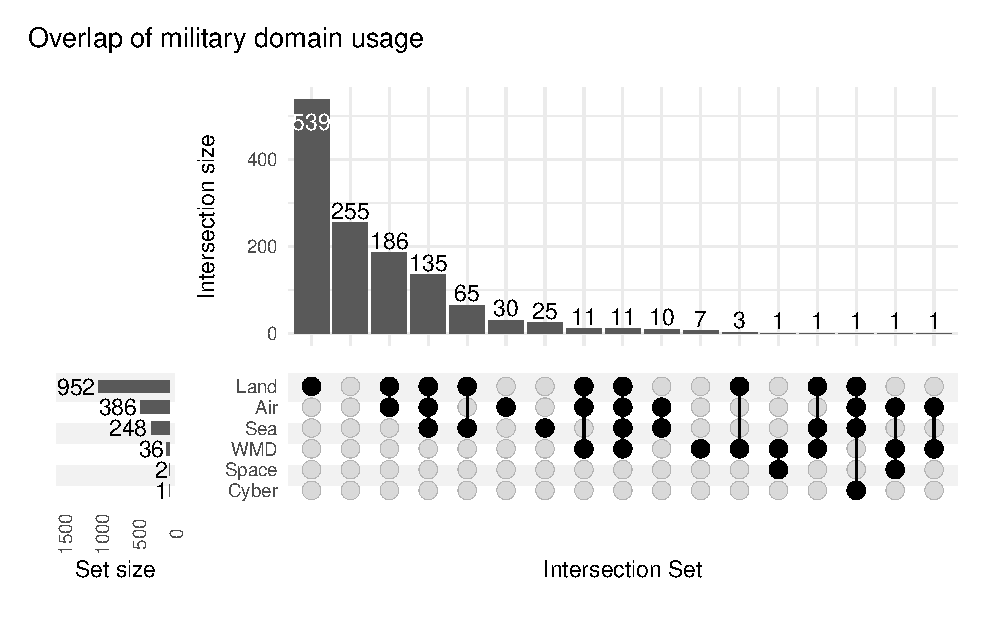
\includegraphics{2022-05-03_ICB-Domains_files/figure-latex/fig-1-1} 

}

\caption{Intersection of domains for each crisis actor. Each bar represents the number of crisis-actors taking military action in the corresponding combination of domains}\label{fig:fig-1}
\end{figure}

\hypertarget{identifying-crisis-dyads}{%
\subsubsection{Identifying crisis-dyads}\label{identifying-crisis-dyads}}

The original ICB data exists at two levels of analysis, the crisis-level and the crisis-actor level. While the actor-level data contains more granularity, it leaves the role of each actor unspecified. So after identifying the military domains in which crisis-actors took actions, this new data was merged with existing data on ICB crisis-dyads (Hewitt 2003; Beardsley and Asal 2009; Levin-Banchik 2020). An ICB crisis-dyad is an ICB crisis in which both sides are sovereign states, at least one state meets the original three ICB crisis conditions, and at least one actor perceives that the other has directed a threat or hostile threat against it. Available crisis-dyad data ends at 2010, so new codings were done for post-2010 crises. The coding followed the same rules and procedures outlined by Hewitt (2003), producing actor-level dyad information for 425 ICB crises.

Numerous crises involve multiple dyads if, for example, military coalitions were involved. To simplify coding, when multiple actors participated on the same side in the conflict, that side was coded as having taken actions in a given military domain if any actor on that side took actions in that domain. For example, if both France and the United States were coded as side A in a crisis and France deployed naval assets and the United States deployed ground forces, side A is simply coded as having taken action in both the naval and land domains.

\hypertarget{measuring-cross-domainness}{%
\subsubsection{Measuring cross-domainness}\label{measuring-cross-domainness}}

The third and final step involves identifying the dissimilarity of the domains in which each side of each crisis-dyad took actions. ``Cross-domainness'' is a continuous variable between 0 and 1, inclusive. For each crisis, if the two sides took actions in identical domains, ``cross-domainess'' equals 0. As the distinctiveness of the domains in which each side acted increases, the value of ``cross-domainness'' increases, with crises where the two sides took actions in entirely distinct domains equaling 1.

This cross-domainness measure is producing by using a Jaccard similarity coefficient to compare the military domains in which each side in a crisis-dyad operated. This measure identifies the union of domains in which each side took actions as a ratio of those in which only one side took action, such that for a crisis-dyad with two sides A and B, \(J_{(A, B)} = \frac{A \cap B}{A + B - (A \cap B)}\). Table \ref{tab:jaccard} provides descriptive examples of how domain similarity in various crises is measured. During its nuclear test in 2009, North Korea launched a satellite followed by an underground nuclear test. The United States, Japan, and South Korea mobilized naval forces as part of military drills and kept interceptor-capable ships in the region following the drills. Since North Korea (side A) took action in the space and WMD domains, while the United States, South Korea, and Japan (side B) responded in the naval domain, the crisis was entirely cross-domain. By contrast, the 1965 Kashmir crisis involving India, Pakistan, and China consisted only of land forces. India (side A) sent troops across the ceasefire line in response to infiltration by Pakistani ``freedom fighters'' (side B). China (also side B) then responded with troop movements near the border. In this case, the crisis was entirely within-domain.

\begin{table}[]
  \centering
  \begin{tabular}{|l|l|cccccc|c|}
  \hline
    \textbf{Crisis} & \textbf{Belligerents} & \multicolumn{1}{l}{\textbf{Land}} & \multicolumn{1}{l}{\textbf{Air}} & \multicolumn{1}{l}{\textbf{Sea}} & \multicolumn{1}{l}{\textbf{WMD}} & \multicolumn{1}{l}{\textbf{Space}} & \multicolumn{1}{l|}{\textbf{Cyber}} & \multicolumn{1}{l|}{\textbf{Jaccard}} \\ 
    \hline
    \multirow{2}{*}{N Korea Nuclear IV (2009)} & US, Japan, S Korea & - & - & 1 & - & - & - & \multirow{2}{*}{1} \\
     & N Korea & - & - & - & 1 & 1 & - & \\
    \hline
    \multirow{2}{*}{Yemen War IV (1967)} & Yemen, Egypt & 1 & 1 & - & 1 & - & - & \multirow{2}{*}{0.67} \\
      & Saudi Arabia & 1 & - & - & - & - & - & \\ 
    \hline
    \multirow{2}{*}{Kashmir I (1947)} & India & 1 & 1 & - & - & - & - & \multirow{2}{*}{0.5} \\
      & Pakistan & 1 & - & - & - & - & - & \\ 
    \hline
    \multirow{2}{*}{Gulf of Tonkin (1964)} & S. Vietnam, U.S. & 1 & 1 & 1 & - & - & - & \multirow{2}{*}{0.33} \\
      & N. Vietnam & 1 & - & 1 & - & - & - & \\ 
    \hline
    \multirow{2}{*}{Kashmir II (1965)} & India & 1 & - & - & - & - & - & \multirow{2}{*}{0} \\
     & Pakistan, China & 1 & - & - & - & - & - & \\ 
    \hline
  \end{tabular}
  \caption{Example of cross-domainness measure at the crisis-level using the Jaccard similarity coefficient. The measure is bounded between 0 and 1, with 0 indicating the two sides took actions in identical domains and 1 meaning complete dissimilarity.}
  \label{tab:jaccard}
  \end{table}

The Jaccard measure is appropriate because each crisis contains precisely two sides (two vectors to compare), the values are binary, and comparison involves the similarity of measures that were employed as opposed to those that were not. Similar measures like the simple matching coefficient (SMC) are less appropriate since there is variation across space and time about what 0's mean (Chung et al. 2019). In some cases, 0's are an omission by choice (states \textit{do not} act in this domain) but in others they represent omission by necessity (states \textit{cannot} act in this domain). Although neither the United States nor Vietnam used WMDs during the Vietnam War, that doesn't make their military strategy similar: the United States could have done so but did not, while Vietnam could not have. Thus, 0's mean different things. This problem is avoided by measuring similarity in terms of what actors actually use, in which domain. This measurement also appropriately tests the theories presented, since they concern the consequences of states interacting in unlike ways. Similar concepts like the number of domains in which actors act are important, but are not the criteria of interest here.

Figure \ref{fig:fig-2} represents the distribution of cross-domainness for all ICB crises. This figure demonstrates that cross-domain military crises are not unusual, just the opposite. Some amount of cross-domain conflict behavior represents the modal form of crisis interaction over the past century. Of the 425 ICB crises, 23\% are entirely cross-domain, meaning the two sides had zero overlap in what military domains they operated in during the crisis, and 58\% had at least some amount of cross-domain interaction. In only 42\% did both sides behave in-kind. Figure \ref{fig:fig-3} shows that the temporal trend of cross-domain interactions runs contrary to conventional wisdom. Despite the common demarcation of the nuclear age and advent of new domains like cyber and space, cross-domain conflict is not an emerging property of new, technological conflict domains (at least not within crises). Although new military tools have become available to states at an arguably ever greater pace, they have not led to an increase in cross-domain activities. Either these domains are not being utilized in international crises, or they are being utilized in about the same way that older domains of conflict were and continue to be exercised. There is no evidence in these data of a transformation of military affairs related to cross-domain conflict. Rather, cross-domain conflict has been, and continues to be, a common feature of conflict behavior generally, at least within crises.

\begin{figure}[h!]

{\centering 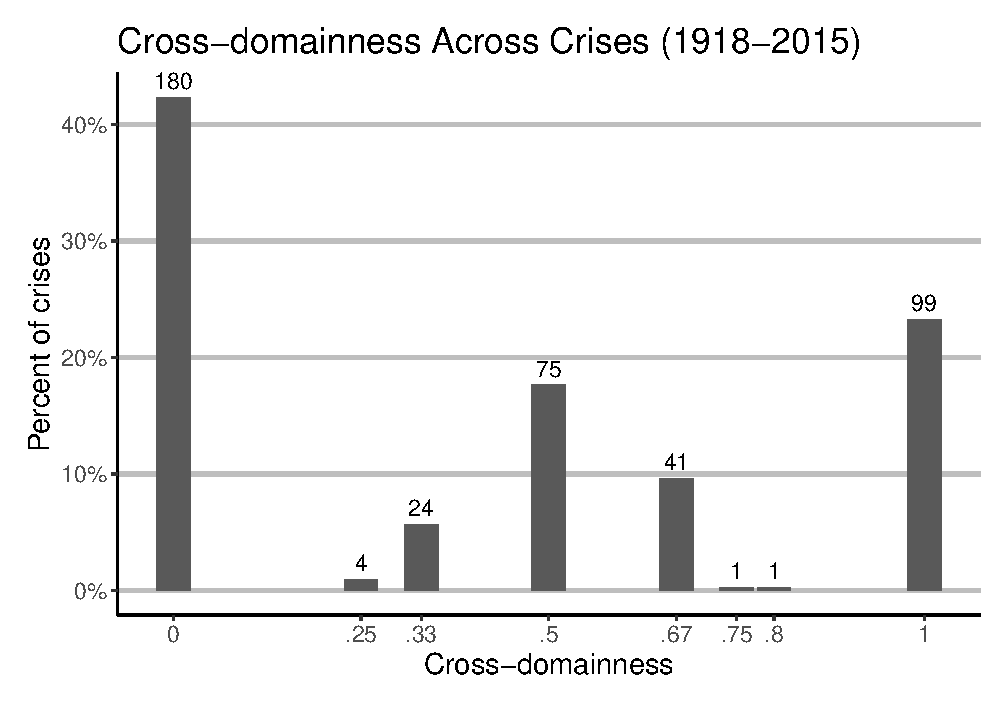
\includegraphics[width=0.8\linewidth,]{2022-05-03_ICB-Domains_files/figure-latex/fig-2-1} 

}

\caption{Distribution of cross-domainness in international crises. Higher x-axis values represent higher cross-domain interactions between adversaries. Numbers above the bars represent number of observations.}\label{fig:fig-2}
\end{figure}

\begin{figure}[h!]

{\centering 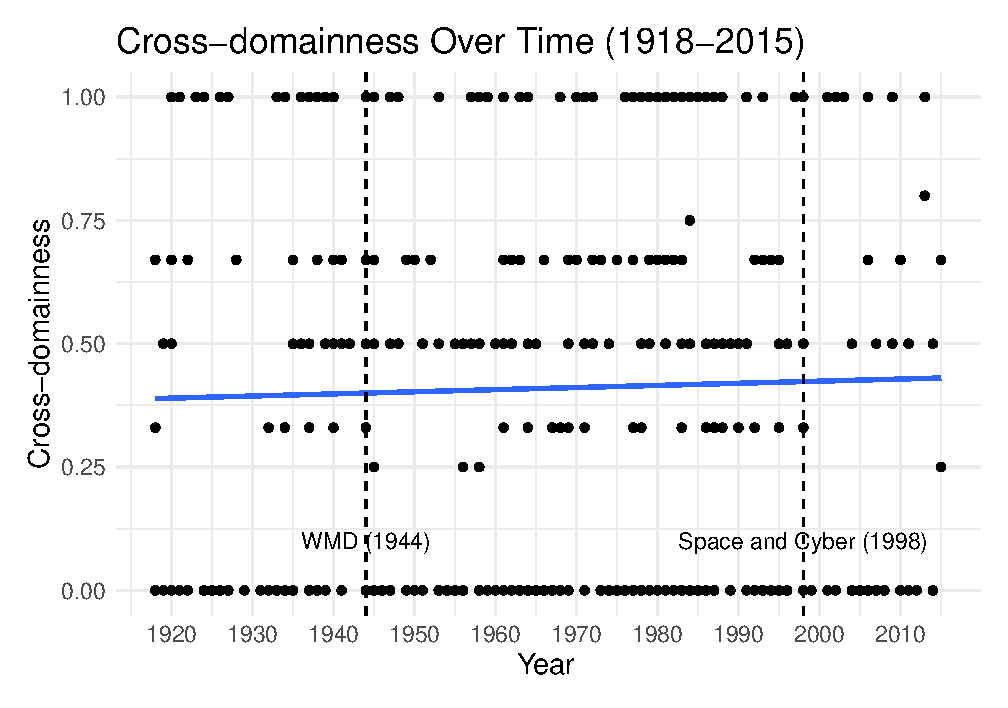
\includegraphics[width=0.8\linewidth,]{2022-05-03_ICB-Domains_files/figure-latex/fig-3-1} 

}

\caption{Distribution of cross-domainness over time. Points represent each observation (ICB crisis) and the line represents a bivariate generalized linear model with the shaded area corresponding to the 95\% confidence interval. The slope is statistically insignificant. The first crises involving land, air, and sea are in the earliest year in the data (1918), while the first crises involving the other domains are labeled.}\label{fig:fig-3}
\end{figure}

\hypertarget{model}{%
\subsection{Model}\label{model}}

To test the hypotheses about a relationship between cross-domain military interactions and crisis escalation, the relationship is modeled using two separate dependent variables --- intensity of violence and crisis duration. These are common observable indicators for conflict escalation and intensity (Allen 2007; Asal and Beardsley 2007). The unit of analysis is the international crisis which has been collapsed down from the crisis-dyad level using the method described above.

Two different model classes are required to estimate the impact of cross-domainness on intensity of violence and crisis duration. The dependent variable for the first model --- intensity of violence --- is measured on an ordinal 1-4 scale with 1 describing no violence and 4 describing-full scale war. The dependent variable for the second model is crisis duration measured in days (median crisis duration is 83 days). Because Model 1 has an ordinal dependent variable, the appropriate model specification is an ordered probit (Johnston, McDonald, and Quist 2020). Model 2 is a duration variable operationalized as the days from crisis initiation to crisis termination, involving a time accelerated hazard model with a log-normal parametric specification (Box-Steffensmeier and Jones 2004). Time accelerated hazard models have been used to estimate factors associated with the duration of interstate or intrastate conflict (Martinez Machain 2015).\footnote{Although other scholars have estimated a Cox proportional hazard model (Allen 2007; Beardsley and Asal 2009), the Schoenfeld residuals for this model (shown in the appendix) show that it fails the proportional hazard assumption test and is thus inappropriate in this instance (Box-Steffensmeier, Reiter, and Zorn 2003).}

One challenge in using the crisis as the unit of analysis is conventional control variables at the actor level cannot be appropriately measured given difficulty in theoretically motivating the appropriate means of aggregation (Petersen, Vasquez, and Wang 2004, 91).\footnote{This includes state-level variables like regime type and dyad-level variables like rivalry. There is a vast and well-developed literature on micro-foundations associated with the intensity and duration of conflict like leader traits. See, among others, McDermott (2004) and Saunders (2009). I bracket discussion of the relationship between individual attributes and the choice of military domains for future research.} Nonetheless, both models include a battery of theoretically grounded control variables that influence the intensity and duration of international crises. The models control for the number of crisis actors; more participants in an international crisis may make it more difficult to bargain peacefully, thus increasing the intensity and duration of a crisis (Petersen, Vasquez, and Wang 2004). There is also a control for whether or not a crisis is part of a protracted conflict. Researchers have hypothesized that ongoing, embedded conflicts lead to more violent crises since they are part of a process that is more difficult to resolve (Azar, Jureidini, and McLaurin 1978).\footnote{ICB defines a protracted conflict as ``an environment of ongoing disputes among adversaries, with fluctuating interaction ranging from violence to near-tranquility, multiple issues and spillover effects on all aspects of their relations, and the absence of mutually-recognized or anticipated termination (the Arab-Israeli conflict, 1947-)'' (Brecher et al. 2020).} The models also control for whether the value that a crisis actor felt was threatened was territorial. Territorial conflicts like border wars are more violent and difficult to resolve (Vasquez and Henehan 2001). Territorial conflicts could also involve more similar capabilities by opposing belligerents since land and air forces may be most relevant in holding or taking territory. The models further include a control for whether the crisis was motivated by ethnic differences since ethnic conflicts have been shown to be more violent and difficult to resolve (Ben-Yehuda and Mishali-Ram 2006). A control is added for the degree of power disparities between each side of a crisis, which is a composite measure of population, GNP, major power alliances, territorial size, military capability, and nuclear capability (Quinn et al. 2006). There is also a control for whether one of the two superpowers, the United States or Soviet Union, was involved in the crisis (Colaresi and Thompson 2002). Lastly, there is a control for contiguity which identifies whether the primary crisis actors share a border (Rasler and Thompson 2006).

\hypertarget{results}{%
\subsection{Results}\label{results}}

The full model results are detailed in Table \ref{tab:model}. For each dependent variable, a bivariate model containing only ``cross-domainness'' as an independent variable is first estimated. Full models that include all control variables are then estimated. For the first two models concerning crisis intensity, the results show that cross-domainness is negatively associated with the intensity of violence with statistical significance at least at the 0.01 standardized level. As the coefficients of ordered logistic regression are difficult to interpret, the odds ratio coefficient for the cross-domainness variable (0.65) indicates that the odds of a crisis with a serious clash or full scale war are 45\% lower than the odds of a crisis containing a minor clash or no violence if the actors use completely dissimilar means.\footnote{A complete table of the odds ratios is provided in the appendix.} These results provide evidence consistent with theories of cross-domain deterrence rather than cross-domain escalation --- crises in which opponents take military actions in dissimilar domains are less violent than those in which opponents take military actions in the same domains.

As models 3 and 4 are parametric time accelerated hazard models, the coefficients detail the likelihood of a crisis ending on a given day. Positive coefficients indicate a variable is associated with a longer crisis while negative coefficients mean the variable is associated with a shorter crisis duration. The coefficients for cross-domainness are negative, but not statistically significant at the 0.01 level once control variables are added to the model. It is not possible to reject the null hypothesis that cross-domainness has no discernible effect on the duration of a crisis. The only statistically significant coefficients for crisis duration relate to the number of crisis actors and ethnic conflict. Both are statistically significant at the 0.01 level and positive, meaning that --- consistent with prior research --- crises with more actors and that are ethnic disputes are longer than crises with fewer actors or that involved other-than-ethnic issues.

\begin{table}[h!]
\begin{center}
\begin{tabular}{l c c c c}
\hline
 & \multicolumn{2}{c}{Violence Intensity} & \multicolumn{2}{c}{Crisis Duration} \\
\cline{2-3} \cline{4-5}
 & Model 1 & Model 2 & Model 3 & Model 4 \\
\hline
Cross-domainness    & $-0.51^{***}$ & $-0.42^{***}$ & $-0.30^{*}$  & $-0.22$      \\
                    & $(0.14)$      & $(0.15)$      & $(0.16)$     & $(0.17)$     \\
No. of actors       &               & $0.08^{***}$  &              & $0.07^{***}$ \\
                    &               & $(0.02)$      &              & $(0.02)$     \\
Power Dissimilarity &               & $-0.00$       &              & $0.00$       \\
                    &               & $(0.00)$      &              & $(0.01)$     \\
Protracted Crisis   &               & $0.28^{**}$   &              & $-0.14$      \\
                    &               & $(0.12)$      &              & $(0.14)$     \\
Territorial Crisis  &               & $0.10$        &              & $0.02$       \\
                    &               & $(0.14)$      &              & $(0.15)$     \\
Major Power Involv. &               & $0.41^{***}$  &              & $0.10$       \\
                    &               & $(0.14)$      &              & $(0.16)$     \\
Ethnic Crisis       &               & $0.17$        &              & $0.65^{***}$ \\
                    &               & $(0.13)$      &              & $(0.15)$     \\
Contiguity          &               & $0.27^{*}$    &              & $-0.04$      \\
                    &               & $(0.15)$      &              & $(0.17)$     \\
Intercept           &               &               & $4.45^{***}$ & $3.82^{***}$ \\
                    &               &               & $(0.09)$     & $(0.22)$     \\
Log (scale)         &               &               & $0.29^{***}$ & $0.24^{***}$ \\
                    &               &               & $(0.03)$     & $(0.04)$     \\
\hline
AIC                 & $1111.83$     & $922.07$      & $5150.51$    & $4471.94$    \\
BIC                 & $1128.05$     & $965.18$      & $5162.67$    & $4511.13$    \\
Log Likelihood      & $-551.91$     & $-450.03$     & $-2572.25$   & $-2225.97$   \\
Deviance            & $1103.83$     & $900.07$      & $$           & $$           \\
Num. obs.           & $426$         & $372$         & $426$        & $372$        \\
\hline
\multicolumn{5}{l}{\scriptsize{\parbox{.75\linewidth}{\vspace{2pt}$^{***}p<0.01$; $^{**}p<0.05$; $^{*}p<0.1$. \\ 
                              Models 1 and 2 are ordered probit models and models 3 and 4 are log-normal accelerated failure time models.}}}
\end{tabular}
\caption{Statistical models}
\label{tab:model}
\end{center}
\end{table}

These findings are robust across a range of alternate modeling decisions detailed in the appendix. Despite the appropriateness of ordered probit and a log-normal parametric specification for the duration model, the results are also consistent using ordered logistic and OLS regression for the severity of violence variable and using other parametric specifications, a Cox proportional hazard model, and OLS for the crisis duration dependent variable. Given the relative rarity of WMD, space, and cyber domains, models are also run with ``cross-domainness'' measured excluding those three domains which produces results consistent with the original model specification. Additional models also are run using a binary dependent variable for violence severity.

Crises in which belligerents interact in dissimilar military domains are less violent, but neither longer nor shorter than crises in which belligerents interact with like-means. While cross-domain conflicts utilizing new modes of conflict have ignited pessimism about potential instability, the empirical evidence provided here should give observers confidence that they can respond to adversarial' ``apples'' with their own ``oranges'' without needing to be overly worried that this decision itself will result in a longer and bloodier contest. As this is a large-n observational study, it is difficult to determine the causal direction of the relationships characterized here. This paper has proposed one mechanism by which cross-domain interactions could reduce the severity and duration of a crisis. The causal arrow may of course run the other way. It could be that the more a state cares about the outcome of a crisis, the more likely the state is to bring its best military assets to the fight. Doing so may in turn cause less blood to be spilled since bringing mobility, stealth, and complexity to the battlefield signals to opponents that discretion may be the better part of valor, lessening violence.

\hypertarget{conclusion}{%
\section{Conclusion}\label{conclusion}}

Emerging interest in understanding cross-domain conflict is well-deserved, given the frequency with which these interactions occur. But this research need not be spurred by, nor limited to, the study of new domains. Crises have always been cross-domain. As far back as World War II, President Roosevelt advocated cross-domain high altitude precision bombing precisely because ``Hitler built a fortress around Europe, but he forgot to put a roof on it.''\footnote{quoted in Grant (2007).} Indeed, contrary to the convictions of many observers, the empirical record suggests cross-domainness has been both common and constant over the past century.

Competing theories of deterrence and spiral models of conflict have rarely accounted for the strategic interaction of the military domains used by opposing sides. The common assumption held by pessimists is cross-domain interactions risk a dangerous spiral because of potential miscommunication over proportionality, stake, and resolve. In contrast, the evidence provided here suggests that cross-domain interactions contain elements of the stability-instability paradox, where one side's willingness to shift conflict new domain --- a potential indicator of a willingness to escalate --- creates conditions that lessen observed crisis escalation.

\newpage

\hypertarget{references}{%
\section*{References}\label{references}}
\addcontentsline{toc}{section}{References}

\hypertarget{refs}{}
\begin{CSLReferences}{1}{0}
\leavevmode\hypertarget{ref-allen_timebombsestimating_2007}{}%
Allen, Susan Hannah. 2007. {``Time {Bombs}: {Estimating} the {Duration} of {Coercive Bombing Campaigns}.''} \emph{Journal of Conflict Resolution} 51 (1): 112--33. \url{https://doi.org/10.1177/0022002706296153}.

\leavevmode\hypertarget{ref-allen_understandingimpactair_2017}{}%
Allen, Susan Hannah, and Carla Martinez Machain. 2017. {``Understanding the Impact of Air Power.''} \emph{Conflict Management and Peace Science} 36 (5): 545--58. \url{https://doi.org/10.1177/0738894216682485}.

\leavevmode\hypertarget{ref-allen_choosingairstrikes_2018}{}%
---------. 2018. {``Choosing {Air Strikes}.''} \emph{Journal of Global Security Studies} 3 (2): 150--62. \url{https://doi.org/10.1093/jogss/ogy005}.

\leavevmode\hypertarget{ref-althaus_clinecenterhistorical_2020}{}%
Althaus, Scott, Joseph Bajjalieh, John Carter, Buddy Peyton, and Dan Shalmon. 2020. {``Cline {Center Historical Phoenix Event Data}.''} {University of Illinois at Urbana-Champaign}: {Cline Center for Advanced Social Research}.

\leavevmode\hypertarget{ref-altman_advancingattackingstrategic_2018}{}%
Altman, Dan. 2018. {``Advancing Without {Attacking}: {The Strategic Game} Around the {Use} of {Force}.''} \emph{Security Studies} 27 (1): 58--88. \url{https://doi.org/10.1080/09636412.2017.1360074}.

\leavevmode\hypertarget{ref-asal_proliferationinternationalcrisis_2007}{}%
Asal, Victor, and Kyle Beardsley. 2007. {``Proliferation and {International Crisis Behavior}.''} \emph{Journal of Peace Research} 44 (2): 139--55. \url{https://doi.org/10.1177/0022343307075118}.

\leavevmode\hypertarget{ref-azar_protractedsocialconflict_1978}{}%
Azar, Edward E., Paul Jureidini, and Ronald McLaurin. 1978. {``Protracted {Social Conflict}; {Theory} and {Practice} in the {Middle East}.''} \emph{Journal of Palestine Studies} 8 (1): 41--60. \url{https://doi.org/10.2307/2536101}.

\leavevmode\hypertarget{ref-beardsley_winningbomb_2009}{}%
Beardsley, Kyle, and Victor Asal. 2009. {``Winning with the {Bomb}.''} \emph{Journal of Conflict Resolution} 53 (2): 278--301. \url{https://doi.org/10.1177/0022002708330386}.

\leavevmode\hypertarget{ref-ben-yehuda_ethnicactorsinternational_2006}{}%
Ben-Yehuda, Hemda, and Meirav Mishali-Ram. 2006. {``Ethnic {Actors} and {International Crises}: {Theory} and {Findings}, 1918{}.''} \emph{International Interactions} 32 (1): 49--78. \url{https://doi.org/10.1080/03050620600584435}.

\leavevmode\hypertarget{ref-borghard_israelrespondedhamas_2019}{}%
Borghard, Erica D., and Jacquelyn Schneider. 2019. {``Israel Responded to a {Hamas} Cyberattack with an Airstrike. {That}'s Not Such a Big Deal.''} \emph{Washington Post}, May.

\leavevmode\hypertarget{ref-box-steffensmeier_eventhistorymodeling_2004}{}%
Box-Steffensmeier, Janet M., and Bradford S. Jones. 2004. \emph{Event {History Modeling}: {A Guide} for {Social Scientists}}. {Cambridge University Press}.

\leavevmode\hypertarget{ref-box-steffensmeier_nonproportionalhazardsevent_2003}{}%
Box-Steffensmeier, Janet M., Dan Reiter, and Christopher Zorn. 2003. {``Nonproportional {Hazards} and {Event History Analysis} in {International Relations}.''} \emph{Journal of Conflict Resolution} 47 (1): 33--53. \url{https://doi.org/10.1177/0022002702239510}.

\leavevmode\hypertarget{ref-brecher_studycrisis_2000}{}%
Brecher, Michael, and Jonathan Wilkenfeld. 2000. \emph{A {Study} of {Crisis}}. {University of Michigan Press}.

\leavevmode\hypertarget{ref-brecher_internationalcrisisbehavior_2020}{}%
Brecher, Michael, Jonathan Wilkenfeld, Kyle C. Beardsley, Patrick James, and David Quinn. 2020. {``International {Crisis Behavior Data Codebook}.''} Codebook Version 14.

\leavevmode\hypertarget{ref-burr_nixonadministrationhorror_2005}{}%
Burr, William. 2005. {``The {Nixon Administration}, the "{Horror Strategy}," and the {Search} for {Limited Nuclear Options}, 1969-1972: {Prelude} to the {Schlesinger Doctrine}.''} \emph{Journal of Cold War Studies} 7 (3): 34--78.

\leavevmode\hypertarget{ref-carson_facingsavingface_2016}{}%
Carson, Austin. 2016. {``Facing {Off} and {Saving Face}: {Covert Intervention} and {Escalation Management} in the {Korean War}.''} \emph{International Organization} 70 (1): 103--31. \url{https://doi.org/10.1017/S0020818315000284}.

\leavevmode\hypertarget{ref-carson_covertcommunicationintelligibility_2017}{}%
Carson, Austin, and Keren Yarhi-Milo. 2017. {``Covert {Communication}: {The Intelligibility} and {Credibility} of {Signaling} in {Secret}.''} \emph{Security Studies} 26 (1): 124--56. \url{https://doi.org/10.1080/09636412.2017.1243921}.

\leavevmode\hypertarget{ref-chung_jaccardtanimotosimilarity_2019}{}%
Chung, Neo Christopher, BłaŻej Miasojedow, Michał Startek, and Anna Gambin. 2019. {``Jaccard/{Tanimoto} Similarity Test and Estimation Methods for Biological Presence-Absence Data.''} \emph{BMC Bioinformatics} 20 (15): 644. \url{https://doi.org/10.1186/s12859-019-3118-5}.

\leavevmode\hypertarget{ref-colaresi_strategicrivalriesprotracted_2002}{}%
Colaresi, Michael P., and William Thompson. 2002. {``Strategic {Rivalries}, {Protracted Conflict}, and {Crisis Escalation}.''} \emph{Journal of Peace Research} 39 (3): 263--87. \url{https://doi.org/10.1177/0022343302039003002}.

\leavevmode\hypertarget{ref-cunningham_maritimerungescalation_2020}{}%
Cunningham, Fiona S. 2020. {``The {Maritime Rung} on the {Escalation Ladder}: {Naval Blockades} in a {US-China Conflict}.''} \emph{Security Studies} 29 (4): 730--68. \url{https://doi.org/10.1080/09636412.2020.1811462}.

\leavevmode\hypertarget{ref-douglass_introducingicbedataset_2022}{}%
Douglass, Rex W., Thomas Leo Scherer, J. Andrés Gannon, Erik Gartzke, Jon Lindsay, Shannon Carcelli, Jonathan Wilkenfeld, et al. 2022. {``Introducing the {ICBe Dataset}: {Very High Recall} and {Precision Event Extraction} from {Narratives} about {International Crises}.''} \emph{arXiv:2202.07081 {[}Cs, Stat{]}}, February. \url{http://arxiv.org/abs/2202.07081}.

\leavevmode\hypertarget{ref-duffield_evolutionnatostrategy_1991}{}%
Duffield, John S. 1991. {``The {Evolution} of {NATO}'s {Strategy} of {Flexible Response}: {A Reinterpretation}.''} \emph{Security Studies} 1 (1): 132--56. \url{https://doi.org/10.1080/09636419109347460}.

\leavevmode\hypertarget{ref-ferreiro_horationelsonnever_2016}{}%
Ferreiro, Larrie D. 2016. {``Horatio {Nelson Never Wrote} {`{A Ship}'s a {Fool} to {Fight} a {Fort}'}; {It Was Jackie Fisher Who Invented} the {Attribution}.''} \emph{Journal of Military History} 80 (3): 855--56.

\leavevmode\hypertarget{ref-gannon_shadowdeterrencewhy_2021}{}%
Gannon, J Andrés, Erik A. Gartzke, Jon R. Lindsay, and Peter Schram. 2021. {``The {Shadow} of {Deterrence}: {Why} Capable Actors Engage in Contests Short of War.''} Working \{\{Paper\}\}.

\leavevmode\hypertarget{ref-gartzke_warerrorterm_1999}{}%
Gartzke, Erik A. 1999. {``War {Is} in the {Error Term}.''} \emph{International Organization} 53 (3): 567--87. \url{https://doi.org/10.1162/002081899550995}.

\leavevmode\hypertarget{ref-gartzke_signalingforeignpolicy_2017}{}%
Gartzke, Erik A., Shannon Carcelli, J Andrés Gannon, and Jiakun Jack Zhang. 2017. {``Signaling in {Foreign Policy}.''} \emph{Oxford Encyclopedia of Foreign Policy Analysis}, August.

\leavevmode\hypertarget{ref-gavin_mythflexibleresponse_2001}{}%
Gavin, Francis J. 2001. {``The {Myth} of {Flexible Response}: {United States Strategy} in {Europe} During the 1960s.''} \emph{The International History Review} 23 (4): 847--75.

\leavevmode\hypertarget{ref-grant_returnbomberfuture_2007}{}%
Grant, Rebecca. 2007. {``Return of the {Bomber}: {The Future} of {Long-Range Strike}.''} {AIR FORCE ASSOCIATION ARLINGTON VA}.

\leavevmode\hypertarget{ref-hewitt_dyadicprocessesinternational_2003}{}%
Hewitt, J. Joseph. 2003. {``Dyadic {Processes} and {International Crises}.''} \emph{Journal of Conflict Resolution} 47 (5): 669--92. \url{https://doi.org/10.1177/0022002703252973}.

\leavevmode\hypertarget{ref-hicks_othermeanspart_2019}{}%
Hicks, Kathleen H., and Alice Hunt Friend. 2019. {``By {Other Means Part I}: {Campaigning} in the {Gray Zone}.''} {Lanham}: {Center for Strategic \& International Studies}.

\leavevmode\hypertarget{ref-horowitz_emergingmilitarytechnologies_2020}{}%
Horowitz, Michael C. 2020. {``Do {Emerging Military Technologies Matter} for {International Politics}?''} \emph{Annual Review of Political Science} 23 (1): 385--400. \url{https://doi.org/10.1146/annurev-polisci-050718-032725}.

\leavevmode\hypertarget{ref-jervis_perceptionmisperceptioninternational_1976}{}%
Jervis, Robert. 1976. \emph{Perception and Misperception in International Politics}. Vol. 49. {Princeton, N.J}: {Princeton University Press}.

\leavevmode\hypertarget{ref-johnston_generalizedorderedprobit_2020}{}%
Johnston, Carla, James McDonald, and Kramer Quist. 2020. {``A Generalized Ordered {Probit} Model.''} \emph{Communications in Statistics - Theory and Methods} 49 (7): 1712--29. \url{https://doi.org/10.1080/03610926.2019.1565780}.

\leavevmode\hypertarget{ref-kreps_escalationfirebreakscyber_2019}{}%
Kreps, Sarah, and Jacquelyn Schneider. 2019. {``Escalation Firebreaks in the Cyber, Conventional, and Nuclear Domains: Moving Beyond Effects-Based Logics.''} \emph{Journal of Cybersecurity} 5 (1): 1--11. \url{https://doi.org/10.1093/cybsec/tyz007}.

\leavevmode\hypertarget{ref-kydd_gametheoryspiral_1997}{}%
Kydd, Andrew. 1997. {``Game {Theory} and the {Spiral Model}.''} \emph{World Politics} 49 (3): 371--400.

\leavevmode\hypertarget{ref-lai_effectsdifferenttypes_2004}{}%
Lai, Brian. 2004. {``The {Effects} of {Different Types} of {Military Mobilization} on the {Outcome} of {International Crises}.''} \emph{The Journal of Conflict Resolution} 48 (2): 211--29.

\leavevmode\hypertarget{ref-levin-banchik_precrisismilitaryhostility_2020}{}%
Levin-Banchik, Luba. 2020. {``Precrisis Military Hostility and Escalation in International Crises.''} \emph{Conflict Management and Peace Science} 38 (1): 63--86. \url{https://doi.org/10.1177/0738894220906376}.

\leavevmode\hypertarget{ref-libicki_cyberspacenotwarfighting_2012}{}%
Libicki, Martin C. 2012. {``Cyberspace {Is Not} a {Warfighting Domain}.''} \emph{I/S: A Journal of Law and Policy for the Information Society} 8: 321.

\leavevmode\hypertarget{ref-lieber_mythnuclearrevolution_2020}{}%
Lieber, Keir A., and Daryl G. Press. 2020. \emph{The {Myth} of the {Nuclear Revolution}: {Power Politics} in the {Atomic Age}}. {Ithaca New York}: {Cornell University Press}.

\leavevmode\hypertarget{ref-lindsay_crossdomaindeterrencestrategy_2019}{}%
Lindsay, Jon R., and Erik A. Gartzke, eds. 2019. \emph{Cross-Domain Deterrence: Strategy in an Era of Complexity}. 1st edition. {New York, NY}: {Oxford University Press}.

\leavevmode\hypertarget{ref-lindsay_politicsmanyother_2020}{}%
---------. 2020. {``Politics by Many Other Means: {The} Comparative Strategic Advantages of Operational Domains.''} \emph{Journal of Strategic Studies} 0 (0): 1--34. \url{https://doi.org/10.1080/01402390.2020.1768372}.

\leavevmode\hypertarget{ref-lupton_signalingresolveleaders_2018}{}%
Lupton, Danielle L. 2018. {``Signaling {Resolve}: {Leaders}, {Reputations}, and the {Importance} of {Early Interactions}.''} \emph{International Interactions} 44 (1): 59--87. \url{https://doi.org/10.1080/03050629.2017.1316268}.

\leavevmode\hypertarget{ref-lupton_reputationalcostsethical_2020}{}%
---------. 2020. {``The {Reputational Costs} and {Ethical Implications} of {Coercive Limited Air Strikes}: {The Fallacy} of the {Middle-Ground Approach}.''} \emph{Ethics \& International Affairs} 34 (2): 217--28. \url{https://doi.org/10.1017/S0892679420000209}.

\leavevmode\hypertarget{ref-macdonald_battlefieldresponsesnew_2019}{}%
Macdonald, Julia, and Jacquelyn Schneider. 2019. {``Battlefield {Responses} to {New Technologies}: {Views} from the {Ground} on {Unmanned Aircraft}.''} \emph{Security Studies} 28 (2): 216--49. \url{https://doi.org/10.1080/09636412.2019.1551565}.

\leavevmode\hypertarget{ref-martinezmachain_aircampaignduration_2015}{}%
Martinez Machain, Carla. 2015. {``Air {Campaign Duration} and the {Interaction} of {Air} and {Ground Forces}.''} \emph{International Interactions} 41 (3): 539--64. \url{https://doi.org/10.1080/03050629.2015.1018414}.

\leavevmode\hypertarget{ref-mastro_signalingmilitaryprovocation_2011}{}%
Mastro, Oriana Skylar. 2011. {``Signaling and {Military Provocation} in {Chinese National Security Strategy}: {A Closer Look} at the {Impeccable Incident}.''} \emph{Journal of Strategic Studies} 34 (2): 219--44. \url{https://doi.org/10.1080/01402390.2011.559025}.

\leavevmode\hypertarget{ref-mawdsley_comparingmilitarieschallenges_2016}{}%
Mawdsley, Jocelyn. 2016. {``Comparing {Militaries}: {The Challenges} of {Datasets} and {Process-Tracing}.''} In \emph{The {Routledge Companion} to {Military Research Methods}}, edited by Alison J. Williams, Neil Jenkings, Rachel Woodward, and Matthew F. Rech, 115--25.

\leavevmode\hypertarget{ref-mcdermott_prospecttheorypolitical_2004}{}%
McDermott, Rose. 2004. {``Prospect {Theory} in {Political Science}: {Gains} and {Losses From} the {First Decade}.''} \emph{Political Psychology} 25 (2): 289--312. \url{https://doi.org/10.1111/j.1467-9221.2004.00372.x}.

\leavevmode\hypertarget{ref-mcmaster_harbingersfuturewar_2016}{}%
McMaster, H. R. 2016. {``Harbingers of {Future War}: {Implications} for the {Army} with {Lieutenant General H}.{R}. {McMaster}.''} {Washington, DC}.

\leavevmode\hypertarget{ref-mehta_extendeddeterrenceassurance_2019}{}%
Mehta, Rupal N. 2019. {``Extended Deterrence and Assurance in an Emerging Technology Environment.''} \emph{Journal of Strategic Studies} 44 (7): 958--82. \url{https://doi.org/10.1080/01402390.2019.1621173}.

\leavevmode\hypertarget{ref-morris_israelgazamilitants_2019}{}%
Morris, Loveday, Ruth Eglash, and Hazem Balousha. 2019. {``Israel and {Gaza} Militants Agree to Cease-Fire After Weekend of Violence.''} \emph{Washington Post}, May.

\leavevmode\hypertarget{ref-morrow_internationallawcommon_2019}{}%
Morrow, James D. 2019. {``International {Law} and the {Common Knowledge Requirements} of {Cross-Domain Deterrence}.''} In \emph{Cross-Domain Deterrence: Strategy in an Era of Complexity}, edited by Jon R. Lindsay and Erik A. Gartzke, 1st edition, 187--204. {New York, NY}: {Oxford University Press}.

\leavevmode\hypertarget{ref-oneill_conflictualmovesbargaining_1991}{}%
O'Neill, Barry. 1991. {``Conflictual Moves in Bargaining: {Warnings}, Threats, Escalations, and Ultimatums.''} In \emph{Negotiation {Analysis}}, edited by H. Peyton Young, 87--108. {University of Michigan Press}.

\leavevmode\hypertarget{ref-petersen_multipartydisputesprobability_2004}{}%
Petersen, Karen K., John A. Vasquez, and Yijia Wang. 2004. {``Multiparty {Disputes} and the {Probability} of {War}, 1816{}.''} \emph{Conflict Management and Peace Science} 21 (2): 85--100. \url{https://doi.org/10.1080/07388940490463898}.

\leavevmode\hypertarget{ref-pettyjohn_competinggrayzone_2019}{}%
Pettyjohn, Stacie L., and Becca Wasser. 2019. {``Competing in the {Gray Zone}: {Russian Tactics} and {Western Responses}.''} {Santa Monica, CA}: {RAND Corporation}.

\leavevmode\hypertarget{ref-post_flyingfailcostly_2019}{}%
Post, Abigail. 2019. {``Flying to {Fail}: {Costly Signals} and {Air Power} in {Crisis Bargaining}.''} \emph{Journal of Conflict Resolution} 63 (4): 869--95. \url{https://doi.org/10.1177/0022002718777043}.

\leavevmode\hypertarget{ref-priebe_fearfrustrationrising_2015}{}%
Priebe, Miranda. 2015. {``Fear and Frustration : Rising State Perceptions of Threats and Opportunities.''} Thesis, Massachusetts Institute of Technology.

\leavevmode\hypertarget{ref-quek_arecostlysignals_2013}{}%
Quek, Kai. 2013. {``Are {Costly Signals More Credible}? {Evidence} from {Three Experiments}.''} \emph{SSRN Electronic Journal}. \url{https://doi.org/10.2139/ssrn.2256528}.

\leavevmode\hypertarget{ref-quinn_powerplaymediation_2006}{}%
Quinn, David, Jonathan Wilkenfeld, Kathleen Smarick, and Victor Asal. 2006. {``Power {Play}: {Mediation} in {Symmetric} and {Asymmetric International Crises}.''} \emph{International Interactions} 32 (4): 441--70. \url{https://doi.org/10.1080/03050620601011107}.

\leavevmode\hypertarget{ref-rasler_contestedterritorystrategic_2006}{}%
Rasler, Karen A., and William R. Thompson. 2006. {``Contested {Territory}, {Strategic Rivalries}, and {Conflict Escalation}.''} \emph{International Studies Quarterly} 50 (1): 145--67. \url{https://doi.org/10.1111/j.1468-2478.2006.00396.x}.

\leavevmode\hypertarget{ref-rovner_giveinstabilitychance_2020}{}%
Rovner, Joshua. 2020. {``Give {Instability} a {Chance}?''} \emph{War on the Rocks}. https://warontherocks.com/2020/07/give-instability-a-chance/.

\leavevmode\hypertarget{ref-saunders_transformativechoicesleaders_2009}{}%
Saunders, Elizabeth N. 2009. {``Transformative {Choices}: {Leaders} and the {Origins} of {Intervention Strategy}.''} \emph{International Security} 34 (2): 119--61. \url{https://doi.org/10.1162/isec.2009.34.2.119}.

\leavevmode\hypertarget{ref-schelling_armsinfluence_1966}{}%
Schelling, Thomas. 1966. \emph{Arms and {Influence}}. {Yale University Press}.

\leavevmode\hypertarget{ref-schrodt_cameoconflictmediation_2005}{}%
Schrodt, Philip A., Deborah Gerner, Ömur Yilmaz, and Dennis Hermreck. 2005. {``The {CAMEO} ({Conflict} and {Mediation Event Observations}) {Actor Coding Framework}.''} In \emph{American {Political Science Association Annual Meeting}}. {Washington, DC}.

\leavevmode\hypertarget{ref-sechser_emergingtechnologiesstrategic_2019}{}%
Sechser, Todd S., Neil Narang, and Caitlin Talmadge. 2019. {``Emerging Technologies and Strategic Stability in Peacetime, Crisis, and War.''} \emph{Journal of Strategic Studies} 42 (6): 727--35. \url{https://doi.org/10.1080/01402390.2019.1626725}.

\leavevmode\hypertarget{ref-slantchev_militarycoercioninterstate_2005}{}%
Slantchev, Branislav L. 2005. {``Military {Coercion} in {Interstate Crises}.''} \emph{American Political Science Review} 99 (4): 533--47. \url{https://doi.org/10.1017/S0003055405051865}.

\leavevmode\hypertarget{ref-talmadge_wouldchinago_2017}{}%
Talmadge, Caitlin. 2017. {``Would {China Go Nuclear}? {Assessing} the {Risk} of {Chinese Nuclear Escalation} in a {Conventional War} with the {United States}.''} \emph{International Security} 41 (4): 50--92. \url{https://doi.org/10.1162/ISEC_a_00274}.

\leavevmode\hypertarget{ref-talmadge_emergingtechnologyintrawar_2019}{}%
---------. 2019. {``Emerging Technology and Intra-War Escalation Risks: {Evidence} from the {Cold War}, Implications for Today.''} \emph{Journal of Strategic Studies} 42 (6): 864--87. \url{https://doi.org/10.1080/01402390.2019.1631811}.

\leavevmode\hypertarget{ref-tan_multidomainbattle_2017}{}%
Tan, Michelle. 2017. {``The {Multi-Domain Battle}.''} \emph{Defense News}. https://www.defensenews.com/digital-show-dailies/ausa/2016/10/03/the-multi-domain-battle/.

\leavevmode\hypertarget{ref-vasquez_territorialdisputesprobability_2001}{}%
Vasquez, John A., and Marie T. Henehan. 2001. {``Territorial {Disputes} and the {Probability} of {War}, 1816-1992.''} \emph{Journal of Peace Research} 38 (2): 123--38.

\leavevmode\hypertarget{ref-warden_limitednuclearwar_2018}{}%
Warden, John K. 2018. {``Limited {Nuclear War}: {The} 21st {Century Challenge} for the {United States}.''} 4. {Lawrence Livermore National Laboratory}: {Center for Global Security Research}.

\end{CSLReferences}

\end{document}
